% ----------------------------------------------------------------------
%  Pracovní úkoly
% ----------------------------------------------------------------------
\section{Pracovní úkoly}

\begin{enumerate}
\item Okalibrujte pomocí bodu tání ledu, bodu varu vody a bodu tuhnutí cínu:
\item[a] platinový odporový teploměr (určete konstanty $R_0, A, B$).
\item[b] termočlánek měď-konstantan (určete konstanty $a, b, c$)

\item Registrujte časový průběh termoelektrického napětí termočlánku $\epsilon(\tau)$ a odporu platinového teploměru $R(\tau)$ při ohřevu a varu vody a při tuhnutí cínu. Změřené průběhy graficky znázorněte.

\item Nakreslete graf teplotní závislosti odporu $R$ (kalibrační křivka odporového teploměru) a graf teplotní závislosti termoelektrického napětí $\epsilon$ (kalibrační křivka termočlánku).

\item Ze závislostí $\epsilon(\tau)$ a $R(\tau)$ dle bodu 2 a kalibračních hodnot dle bodu 1 určete časové závislosti $t_R(T)$ a $t_\epsilon(T)$ teplot měřených odporovým teploměrem a termočlánkem při ohřevu vody a tuhnutí cínu. Určené závislosti porovnejte.

\end{enumerate}

% ----------------------------------------------------------------------
%  Teoretická část
% ----------------------------------------------------------------------
\section{Teoretická část}
Fázové přechody jsou děje, při kterých látka přechází z jednoho skupenství do jiného. U chemicky čistých látek pozorujeme během fázového přechodu oblast s konstantní teplotou v časové závislosti, kde dochází ke změně skupenství (fáze). U ostatních látek se tato teplota o určitou hodnotu mění.

\textbf{Termočlánek} je složen ze dvou různých kovových vodičů. Tyto vodiče jsou na konci svařené. Podle složení těchto vodičů provádíme kalibraci. Aparatura termočlánku je zobrazena na obrázku \ref{fig:aparatura-termoclanku} podle [1]. Oblast $S_1$ je srovnávací známé teploty $t_1$. Teplota $t_2$ je měřená teplota. Výhodou je malá tepelná kapacita a tedy nízké ovlivnění teploty měřeného vzorku.

\begin{figure}[h]
    \centering
    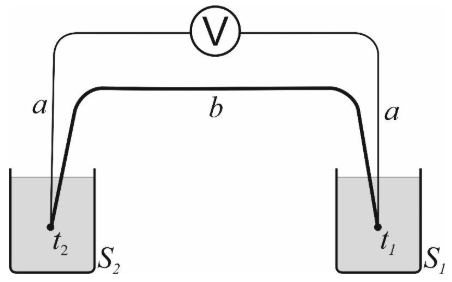
\includegraphics[width=0.5\linewidth]{8 - Kalibrace odporového teploměru a termočlánku//Prototkol - kalibrace teploměru//img/Aparatura termočlánku.png}
    \caption{Aparatura termočlánku}
    \label{fig:aparatura-termoclanku}
\end{figure}

\textbf{Odporový teploměr} měří na základě změny odporu kovu s teplotou. Standardní používané teploměry se vyrábějí z platiny.

V této práci určujeme konstanty $R_0, A, B, a, b, c$ v rovnicích, které popisují závislosti těchto dějů. Pro termočlánek platí v nejjednodušším případě aproximativní kvadratická teplotní závislost

\begin{equation}
    \epsilon = a + b(t_2 - t_1) + c(t_2 - t_1)^2
\end{equation}

kde $\epsilon$ je termoelektrické napětí a $(t_2 - t_1)$ je rozdíl teplot na obou koncích vodičů termočlánku.

Pro platinový odporový teploměr platí závislost odporu $R$ na teplotě $t$ platí

\begin{equation}
    R = R_0 (1 + At + Bt^2)
\end{equation}

Teplotu varu vody je možné vyjádřit jako

\begin{equation}
    t_p = 100 + 28,0216 \left( \frac{p}{p_0} - 1 \right) - 11,642 \left( \frac{p}{p_0} - 1 \right)^2 + 7,1 \left( \frac{p}{p_0} - 1 \right)^3
\end{equation}

kde $p_0$ je normální atmosférický tlak $p_0 = 1,01325 \cdot 10^5 Pa$ a $p$ naměřený tlak.

% ----------------------------------------------------------------------
%  Výsledky a zpracování měření
% ----------------------------------------------------------------------
\section{Výsledky a zpracování měření}

\subsection{Laboratorní podmínky}

    Měření bylo prováděno za laboratorních podmínek uvedených v tabulce \ref{tab:lab_pod}. Pro nás je, ale důležitý naměřený tlak, který ovlivňuje například teplotu varu vody.

    \begin{table}[h]
        \centering
        \begin{tabular}{|c|c|c|} 
        \hline
            t / °C & p / hPa & vlhkost / \%RH  \\ 
        \hline
            23,5(4)   & 984(2)   & 37(3)            \\
        \hline
        \end{tabular}
        \caption{Laboratorní podmínky}
        \label{tab:lab_pod}
    \end{table}

\subsection{Tání ledu}
Nejprve změříme odpor při teplotě $0 \; ^\circ C$. Umístíme směs ledu a vody do termosky a měříme vzniklé termoelektrické napětí a zaznamenáváme odpor po časových intervalech. Čekáme, než se ustálí hodnota odporu. Teplota této směsy je právě $0 ^\circ C$, proto ustálená hodnota odporu odpovídá hodnotě $R_0$ z rovnice (2). Pro odporový teploměr dostáváme $R_0 = 101,0(5) \; \Omega$. Nepřesnost měření odporu je 0,5 \% plus 0,1 \% z rozsahu. Tato závislost je zobrazena na obrázku \ref{fig:odpor-na-teplote-led}.

\begin{figure}[h]
    \centering
    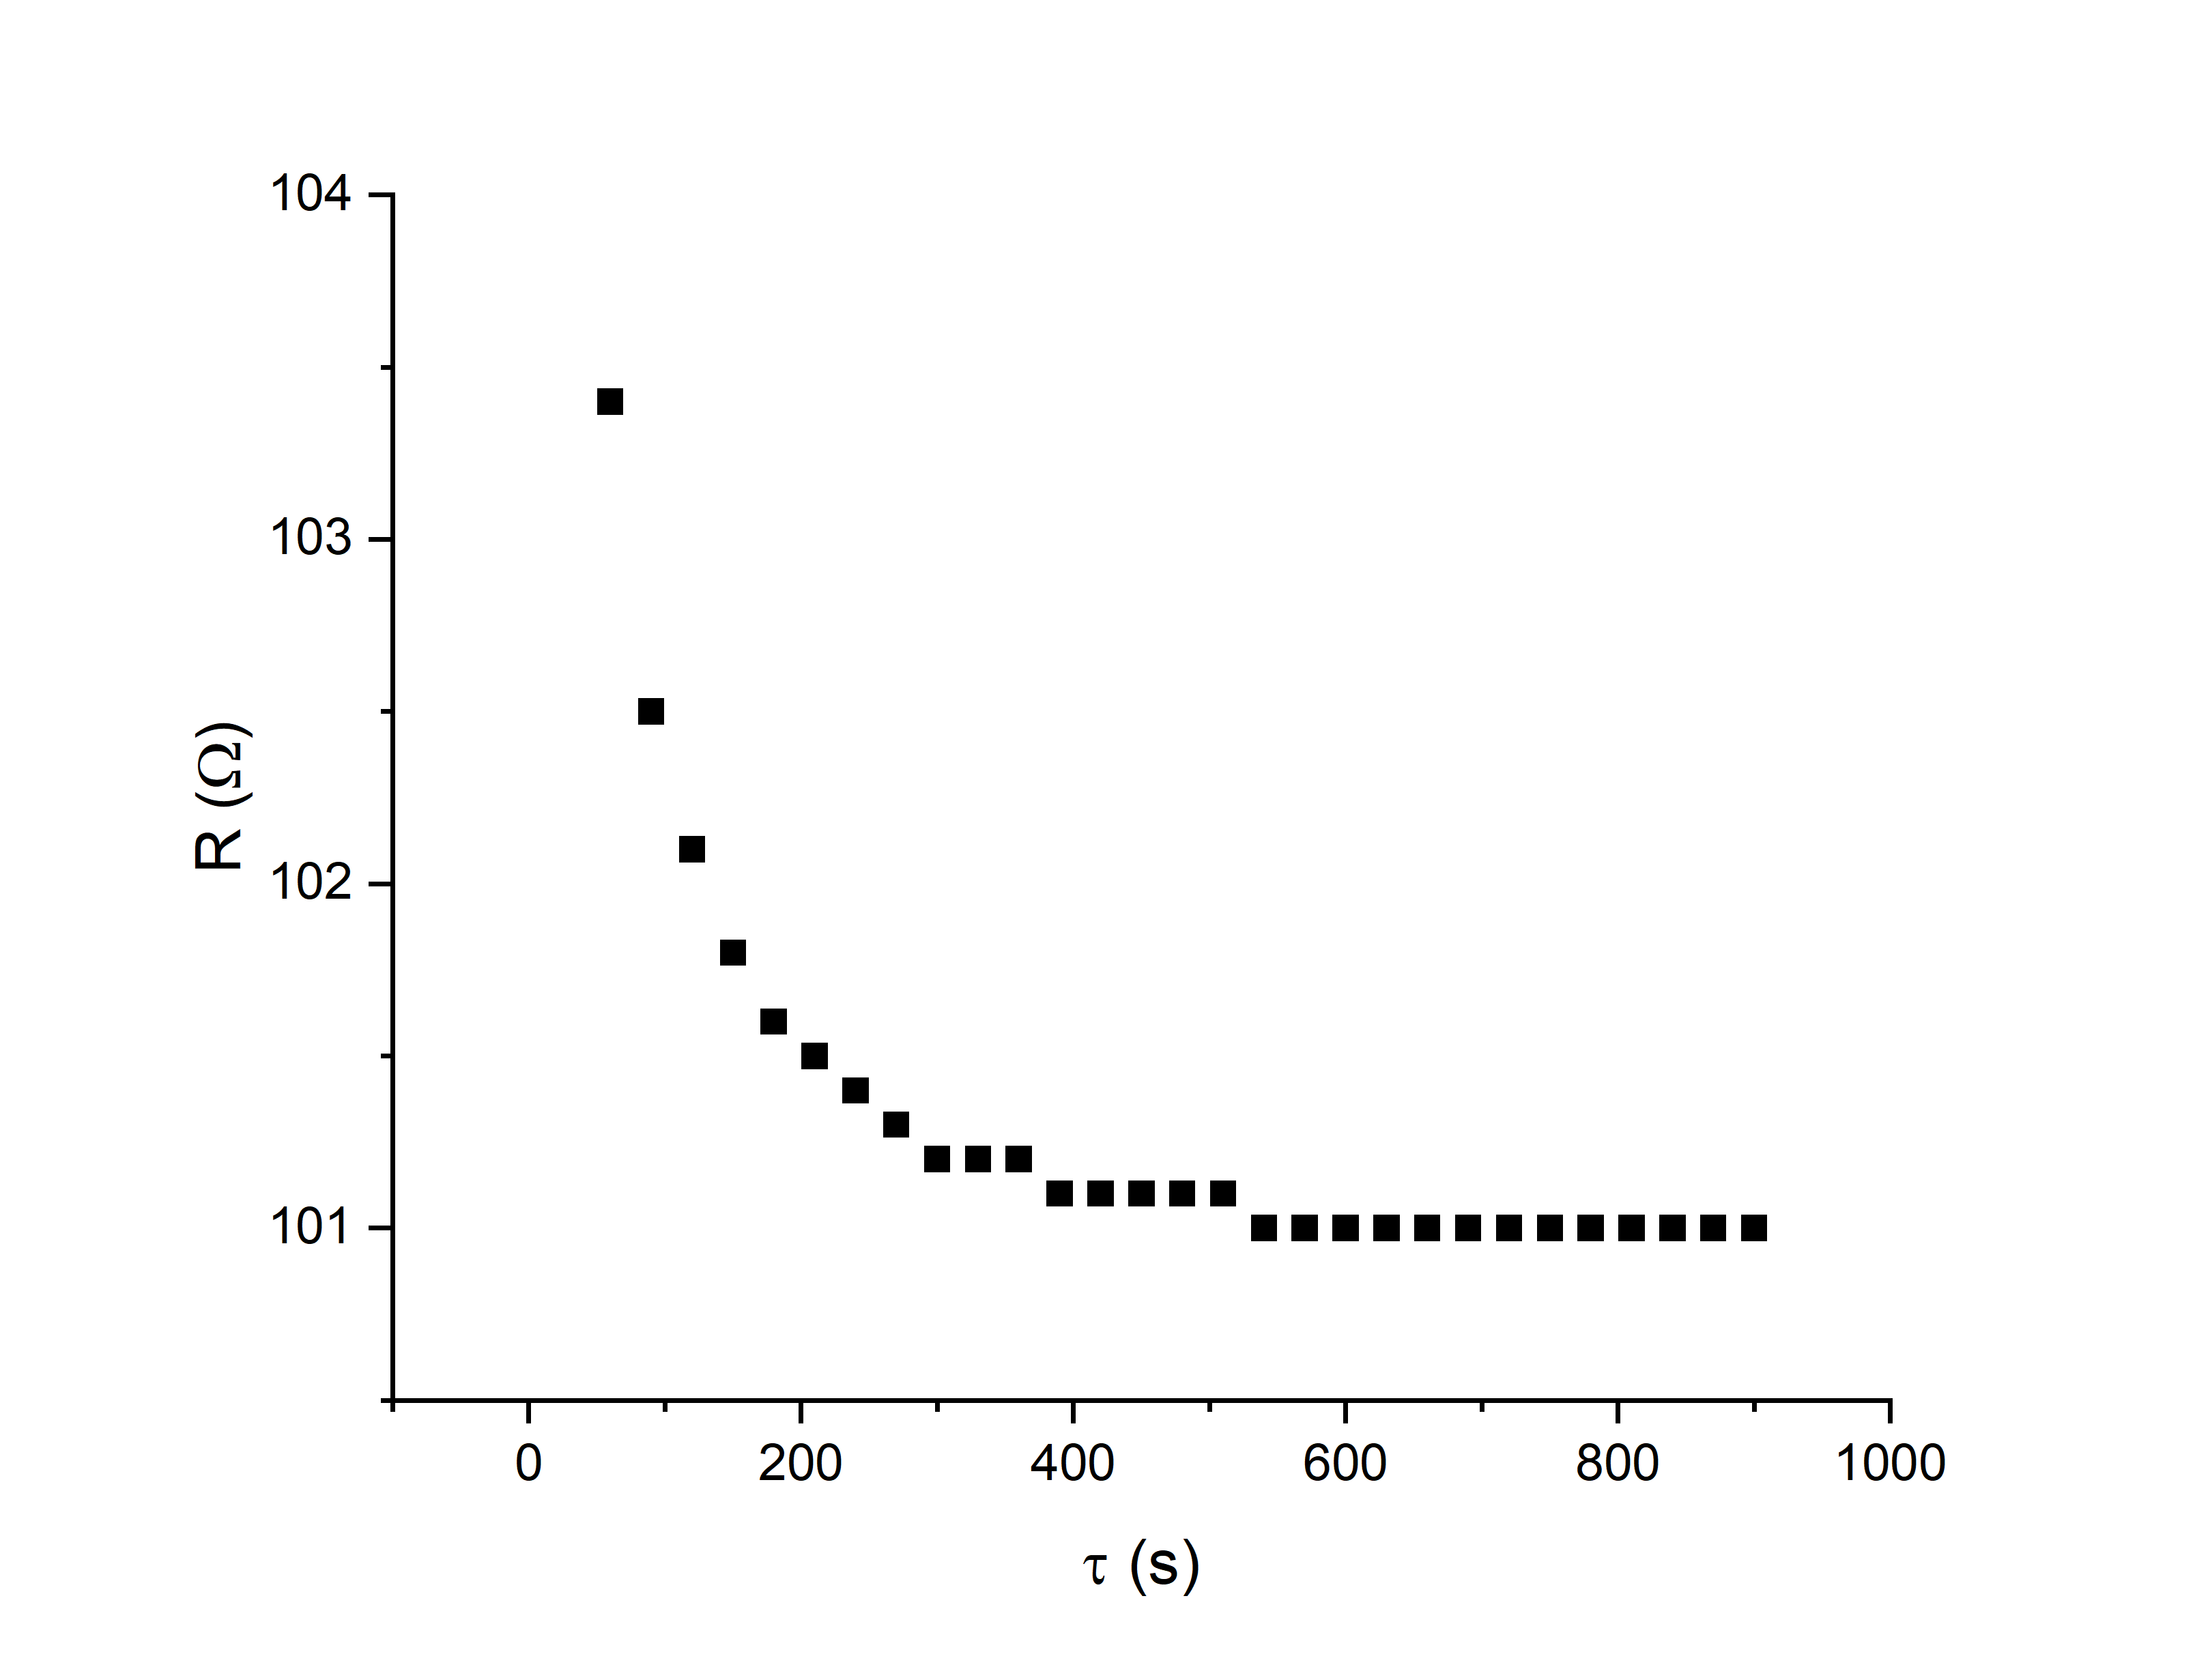
\includegraphics[width=0.5\linewidth]{8 - Kalibrace odporového teploměru a termočlánku//Prototkol - kalibrace teploměru//img/Závislost R na t, tání ledu.png}
    \caption{Závislost odporu na čase pro tání ledu}
    \label{fig:odpor-na-teplote-led}
\end{figure}

Pro termočlánek při rozdílu teplot $0 \; ^\circ C$ dostáváme $\epsilon = 1,4(2) \cdot 10^{-6} \; V$. Udávaná chyba zařízení je 90 ppm z měření a 35 ppm z rozsahu. Závislost je promítnuta do grafu.




\subsection{Var vody}

Jeden konec vodiče termočlánku necháme v termosce, která má teplotu $t_1 = 0 \; ^\circ C$. Druhý konec umístíme nad zahřívanou vodu. Hodnota varu vody je závislá na atmosférickém tlaku, kterou spočteme podle (3) dosazením laboratorního tlaku

\begin{equation}
    \nonumber
    t_p = 99,2(4) \; ^\circ C
\end{equation}

kde nejistota je odhadnuta podle metody přenosu chyb.

Pro odporový teploměr dostáváme při teplotě varu $R = 138,5(7) \; \Omega$. Tato závislost je zobrazena na grafu \ref{fig:odpor-na-teplote-var}.

\begin{figure}[h]
    \centering
    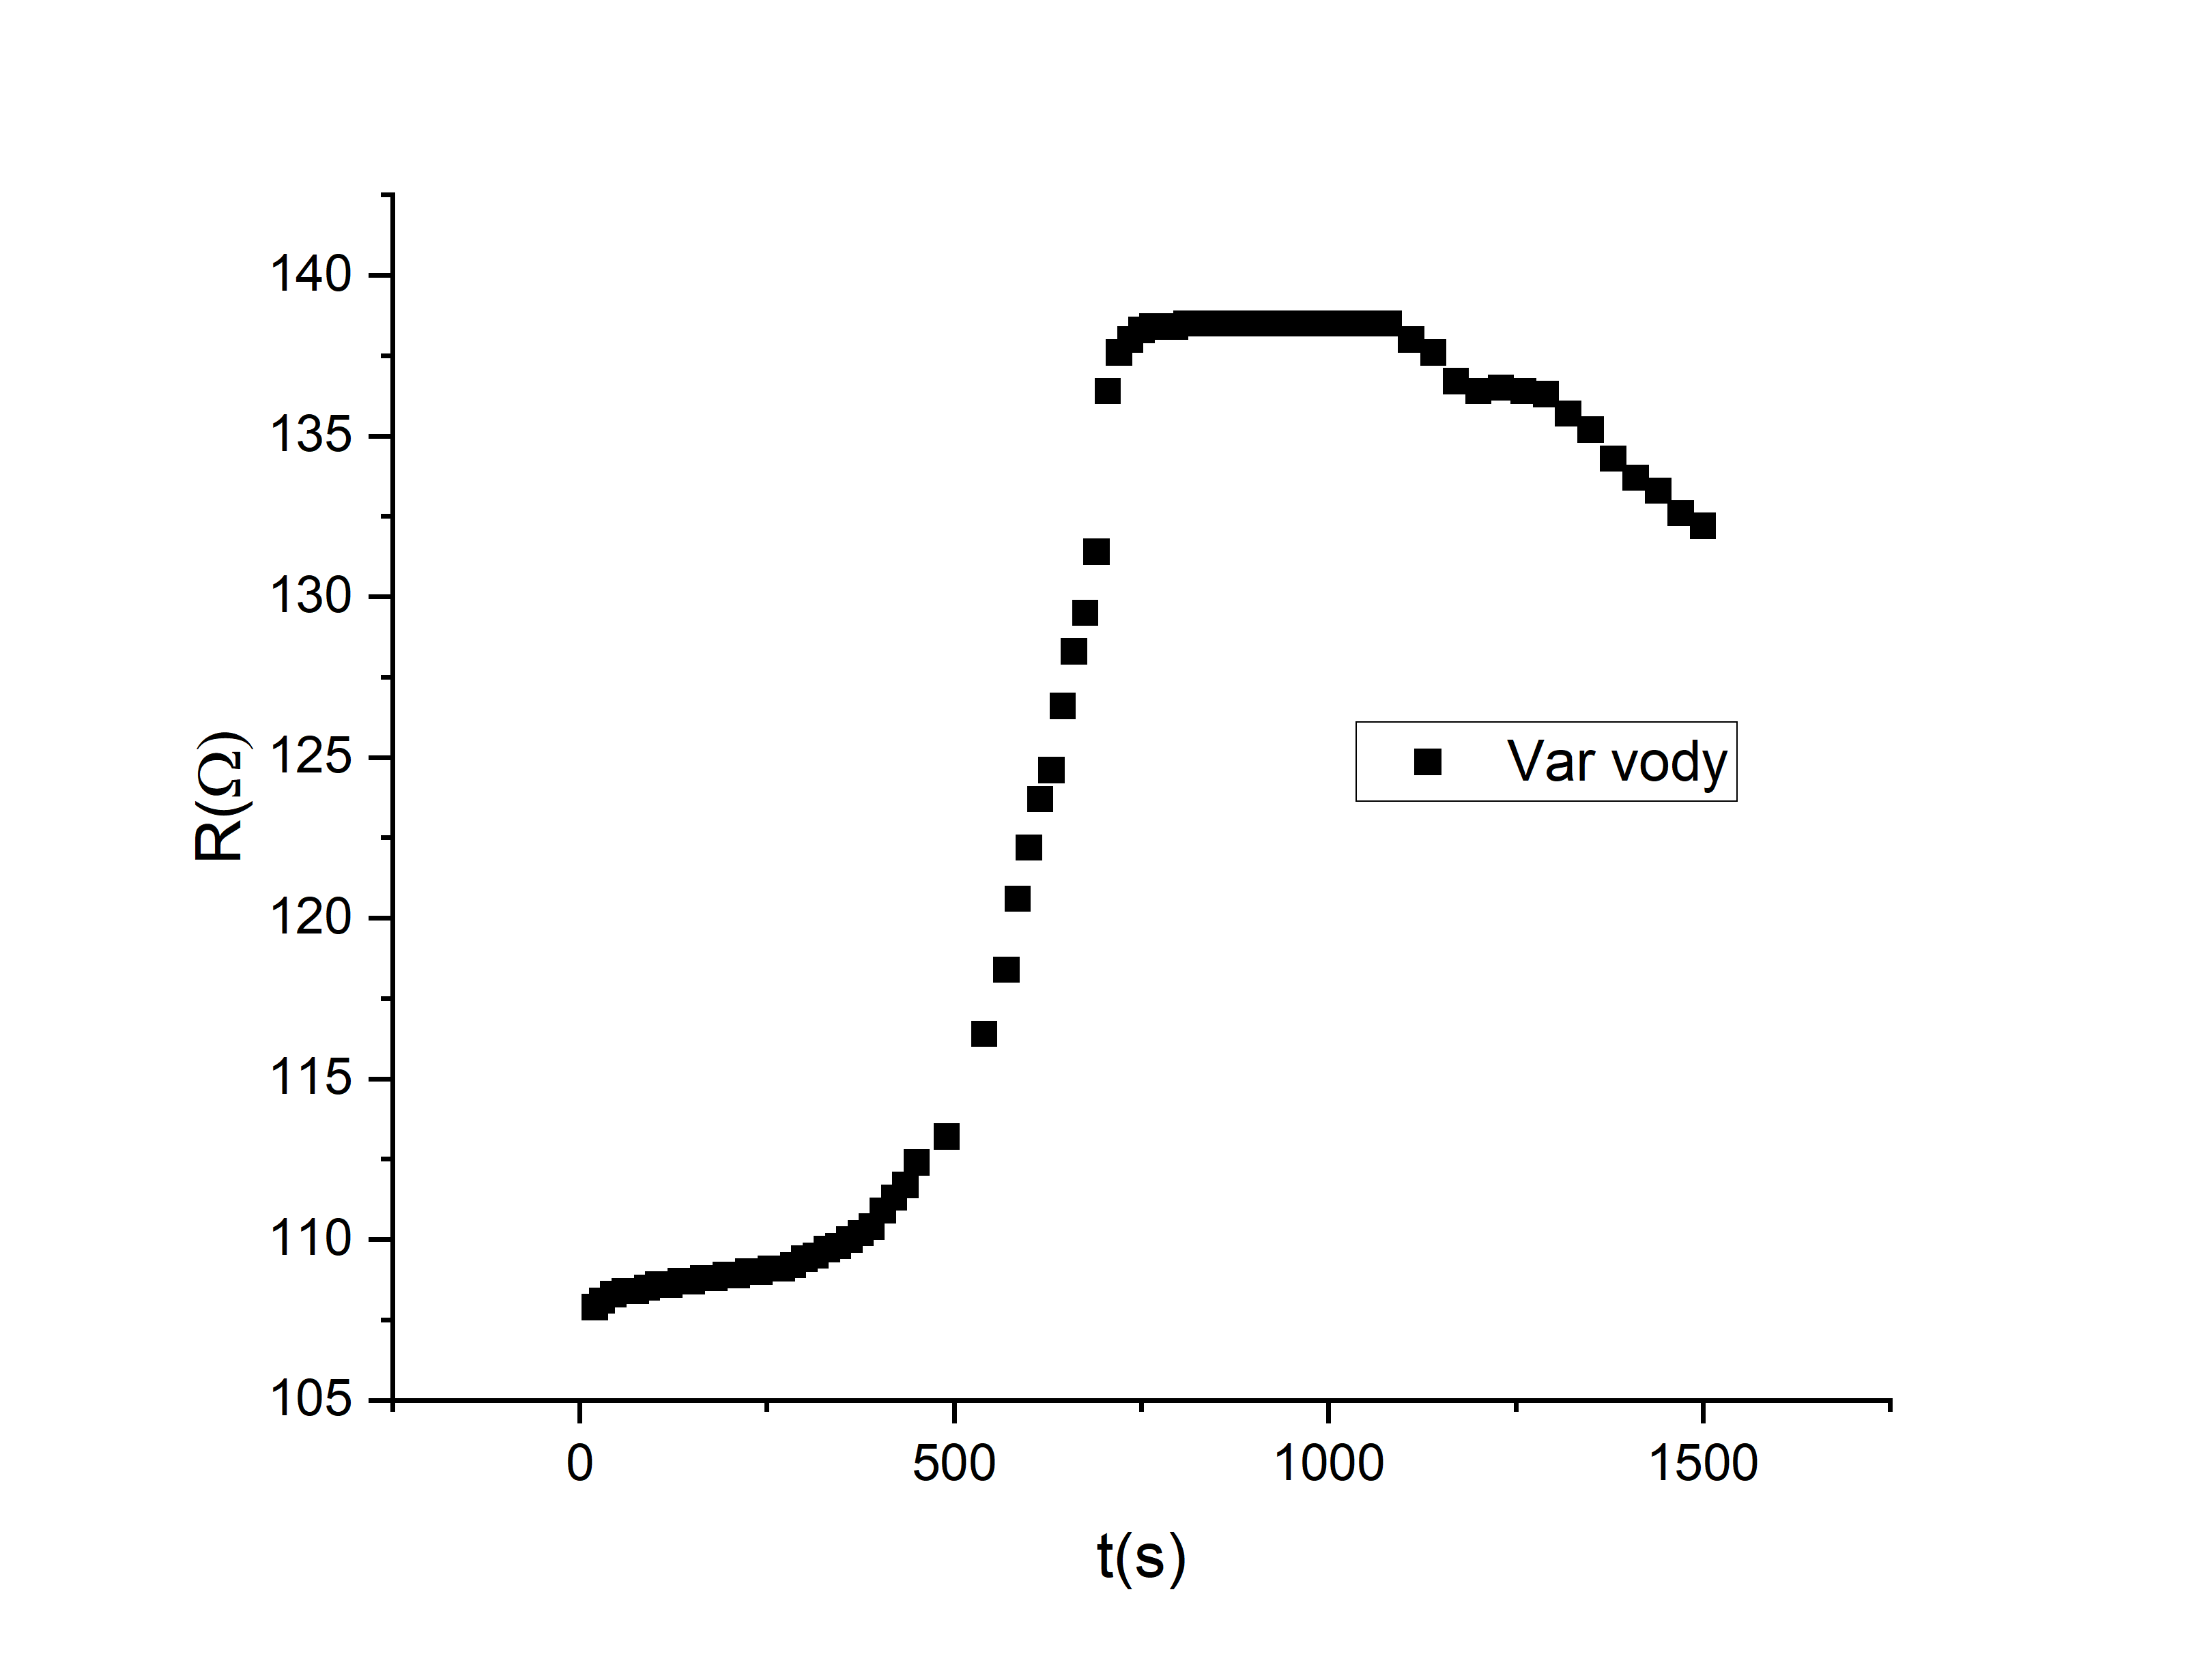
\includegraphics[width=0.5\linewidth]{8 - Kalibrace odporového teploměru a termočlánku//Prototkol - kalibrace teploměru//img/Závislost R na t, var vody.png}
    \caption{Závislost odporu na čase pro var vody}
    \label{fig:odpor-na-teplote-var}
\end{figure}

Pro termočlánek dostáváme při rozdílu teplot odpovídající teplotě varu hodnotu $\epsilon = 4,24(5) \cdot 10^{-4} \; V$.

\newpage
\subsection{Tavení cínu}

Bod tuhnutí cínu nastává při teplotě $t_c = 232 \; ^\circ C$. Hodnota odporu je při této teplotě rovna $R = 187,1(9) \; \Omega$. Hodnota $\epsilon = 1,095(1) \cdot 10^{-2} \; V$. Závislost odporu na čase je v grafu \ref{fig:odpor-na-teplote-cin}.

\begin{figure}[h]
    \centering
    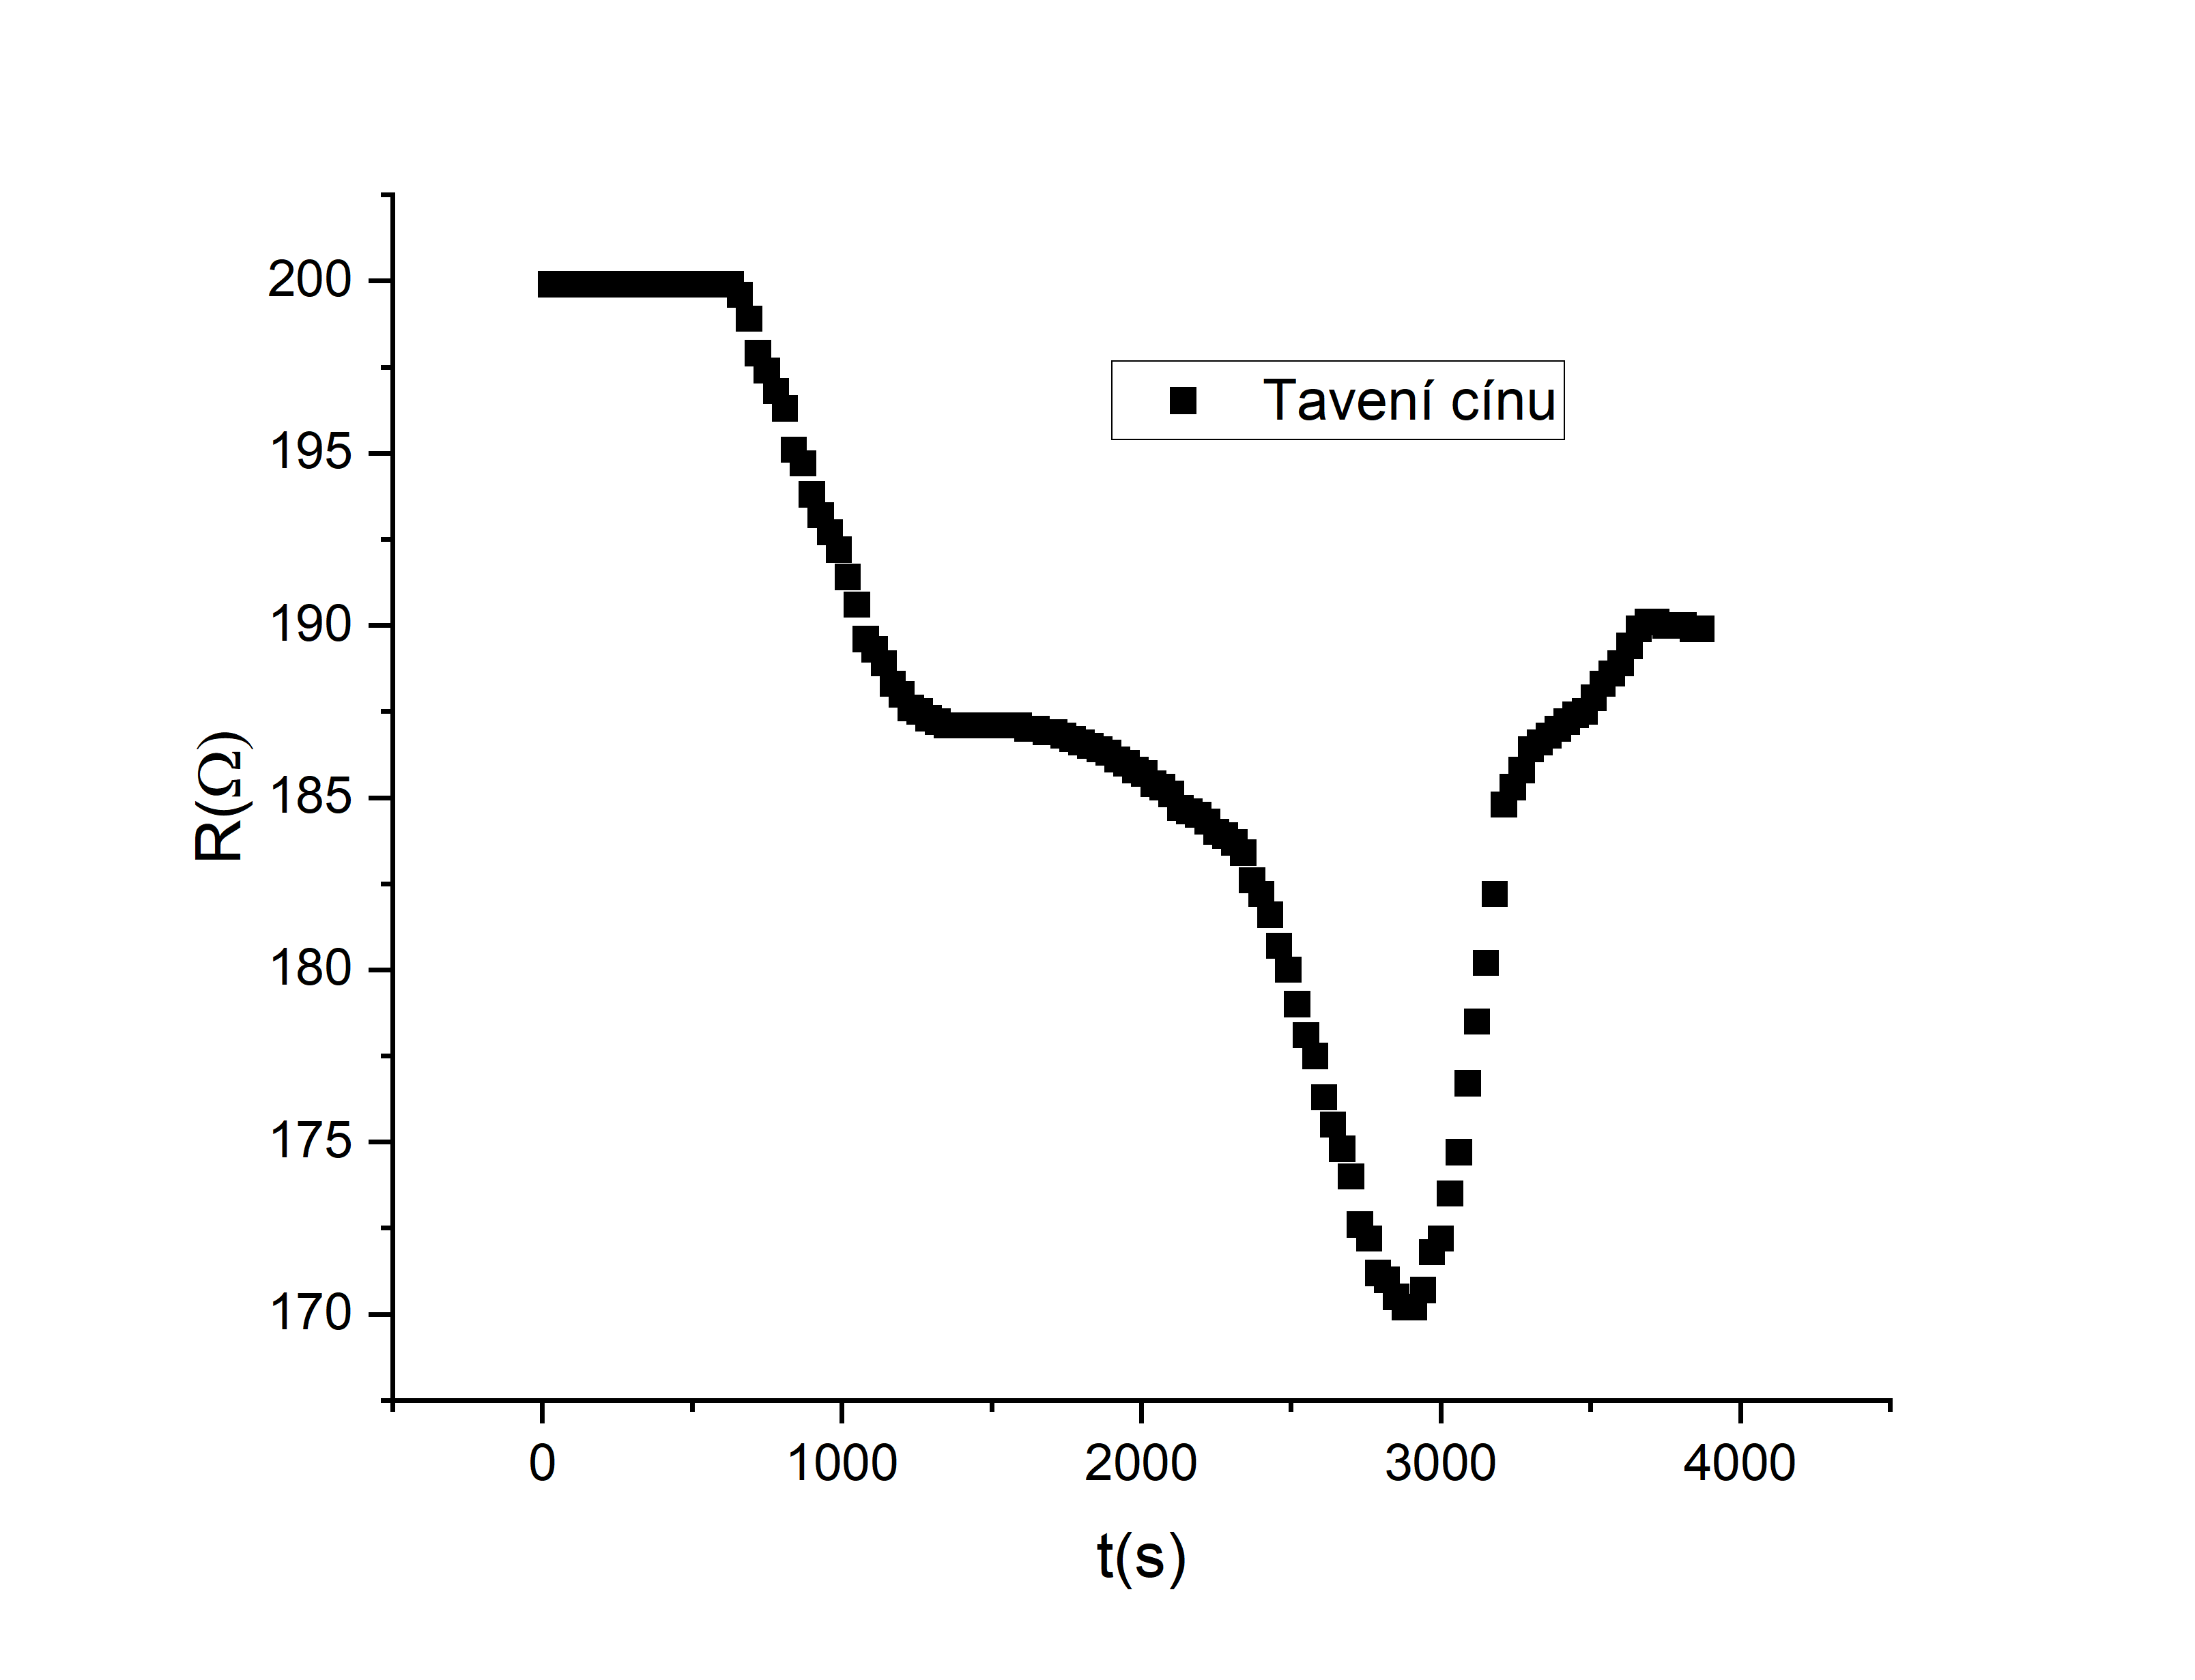
\includegraphics[width=0.5\linewidth]{8 - Kalibrace odporového teploměru a termočlánku//Prototkol - kalibrace teploměru//img/Závislost R na t, tavení cínu.png}
    \caption{Závislost odporu na čase pro tavení cínu}
    \label{fig:odpor-na-teplote-cin}
\end{figure}

\subsection{Kalibrační křivky}
Z naměřených hodnot odporu na napětí můžeme sestavit kalibrační křivku. Hodnoty jsou zaneseny do grafu \ref{fig:krivka-odpor} odporového teploměru a \ref{fig:krivka-termoclanek} termočlánku a je zde také sestrojen polynomiální fit se stupněm 2. Odtud získáme hledané konstanty.

\begin{figure}[h]
    \centering
    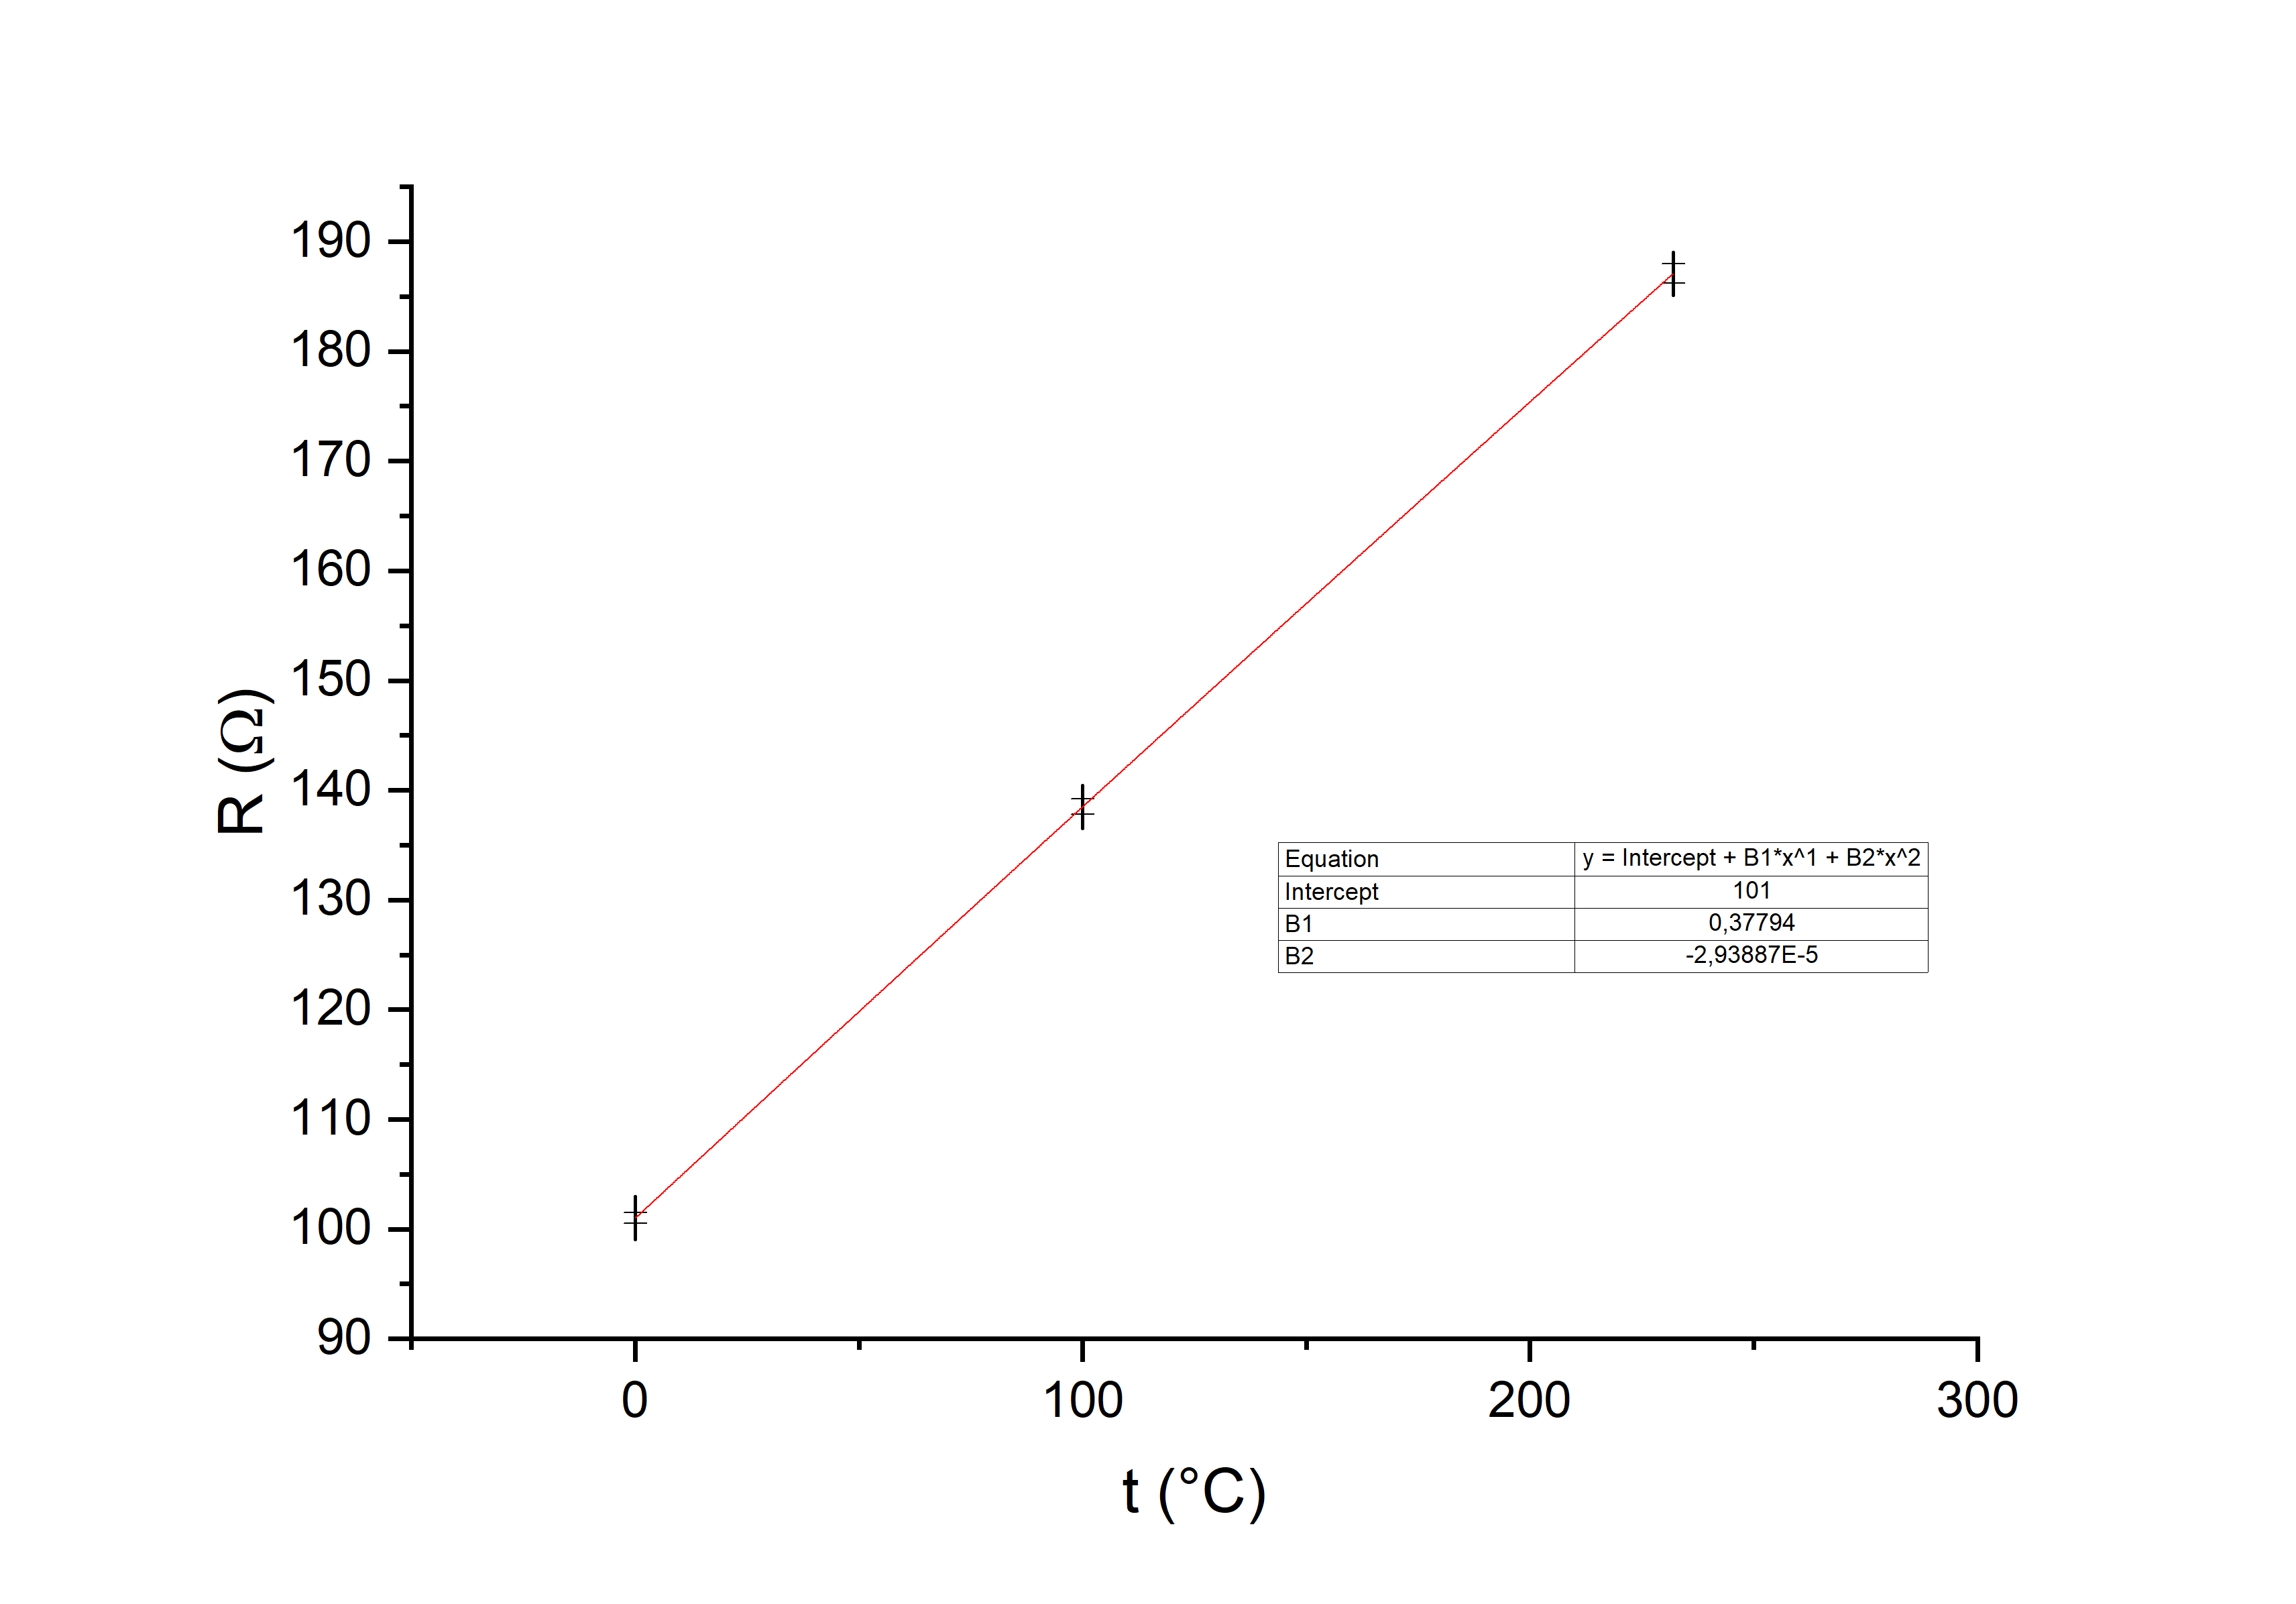
\includegraphics[width=0.8\linewidth]{8 - Kalibrace odporového teploměru a termočlánku//Prototkol - kalibrace teploměru//img/Závislost R na t, parabola.png}
    \caption{Kalibrační křivka pro odporový teploměr}
    \label{fig:krivka-odpor}
\end{figure}

\begin{figure}[h]
    \centering
    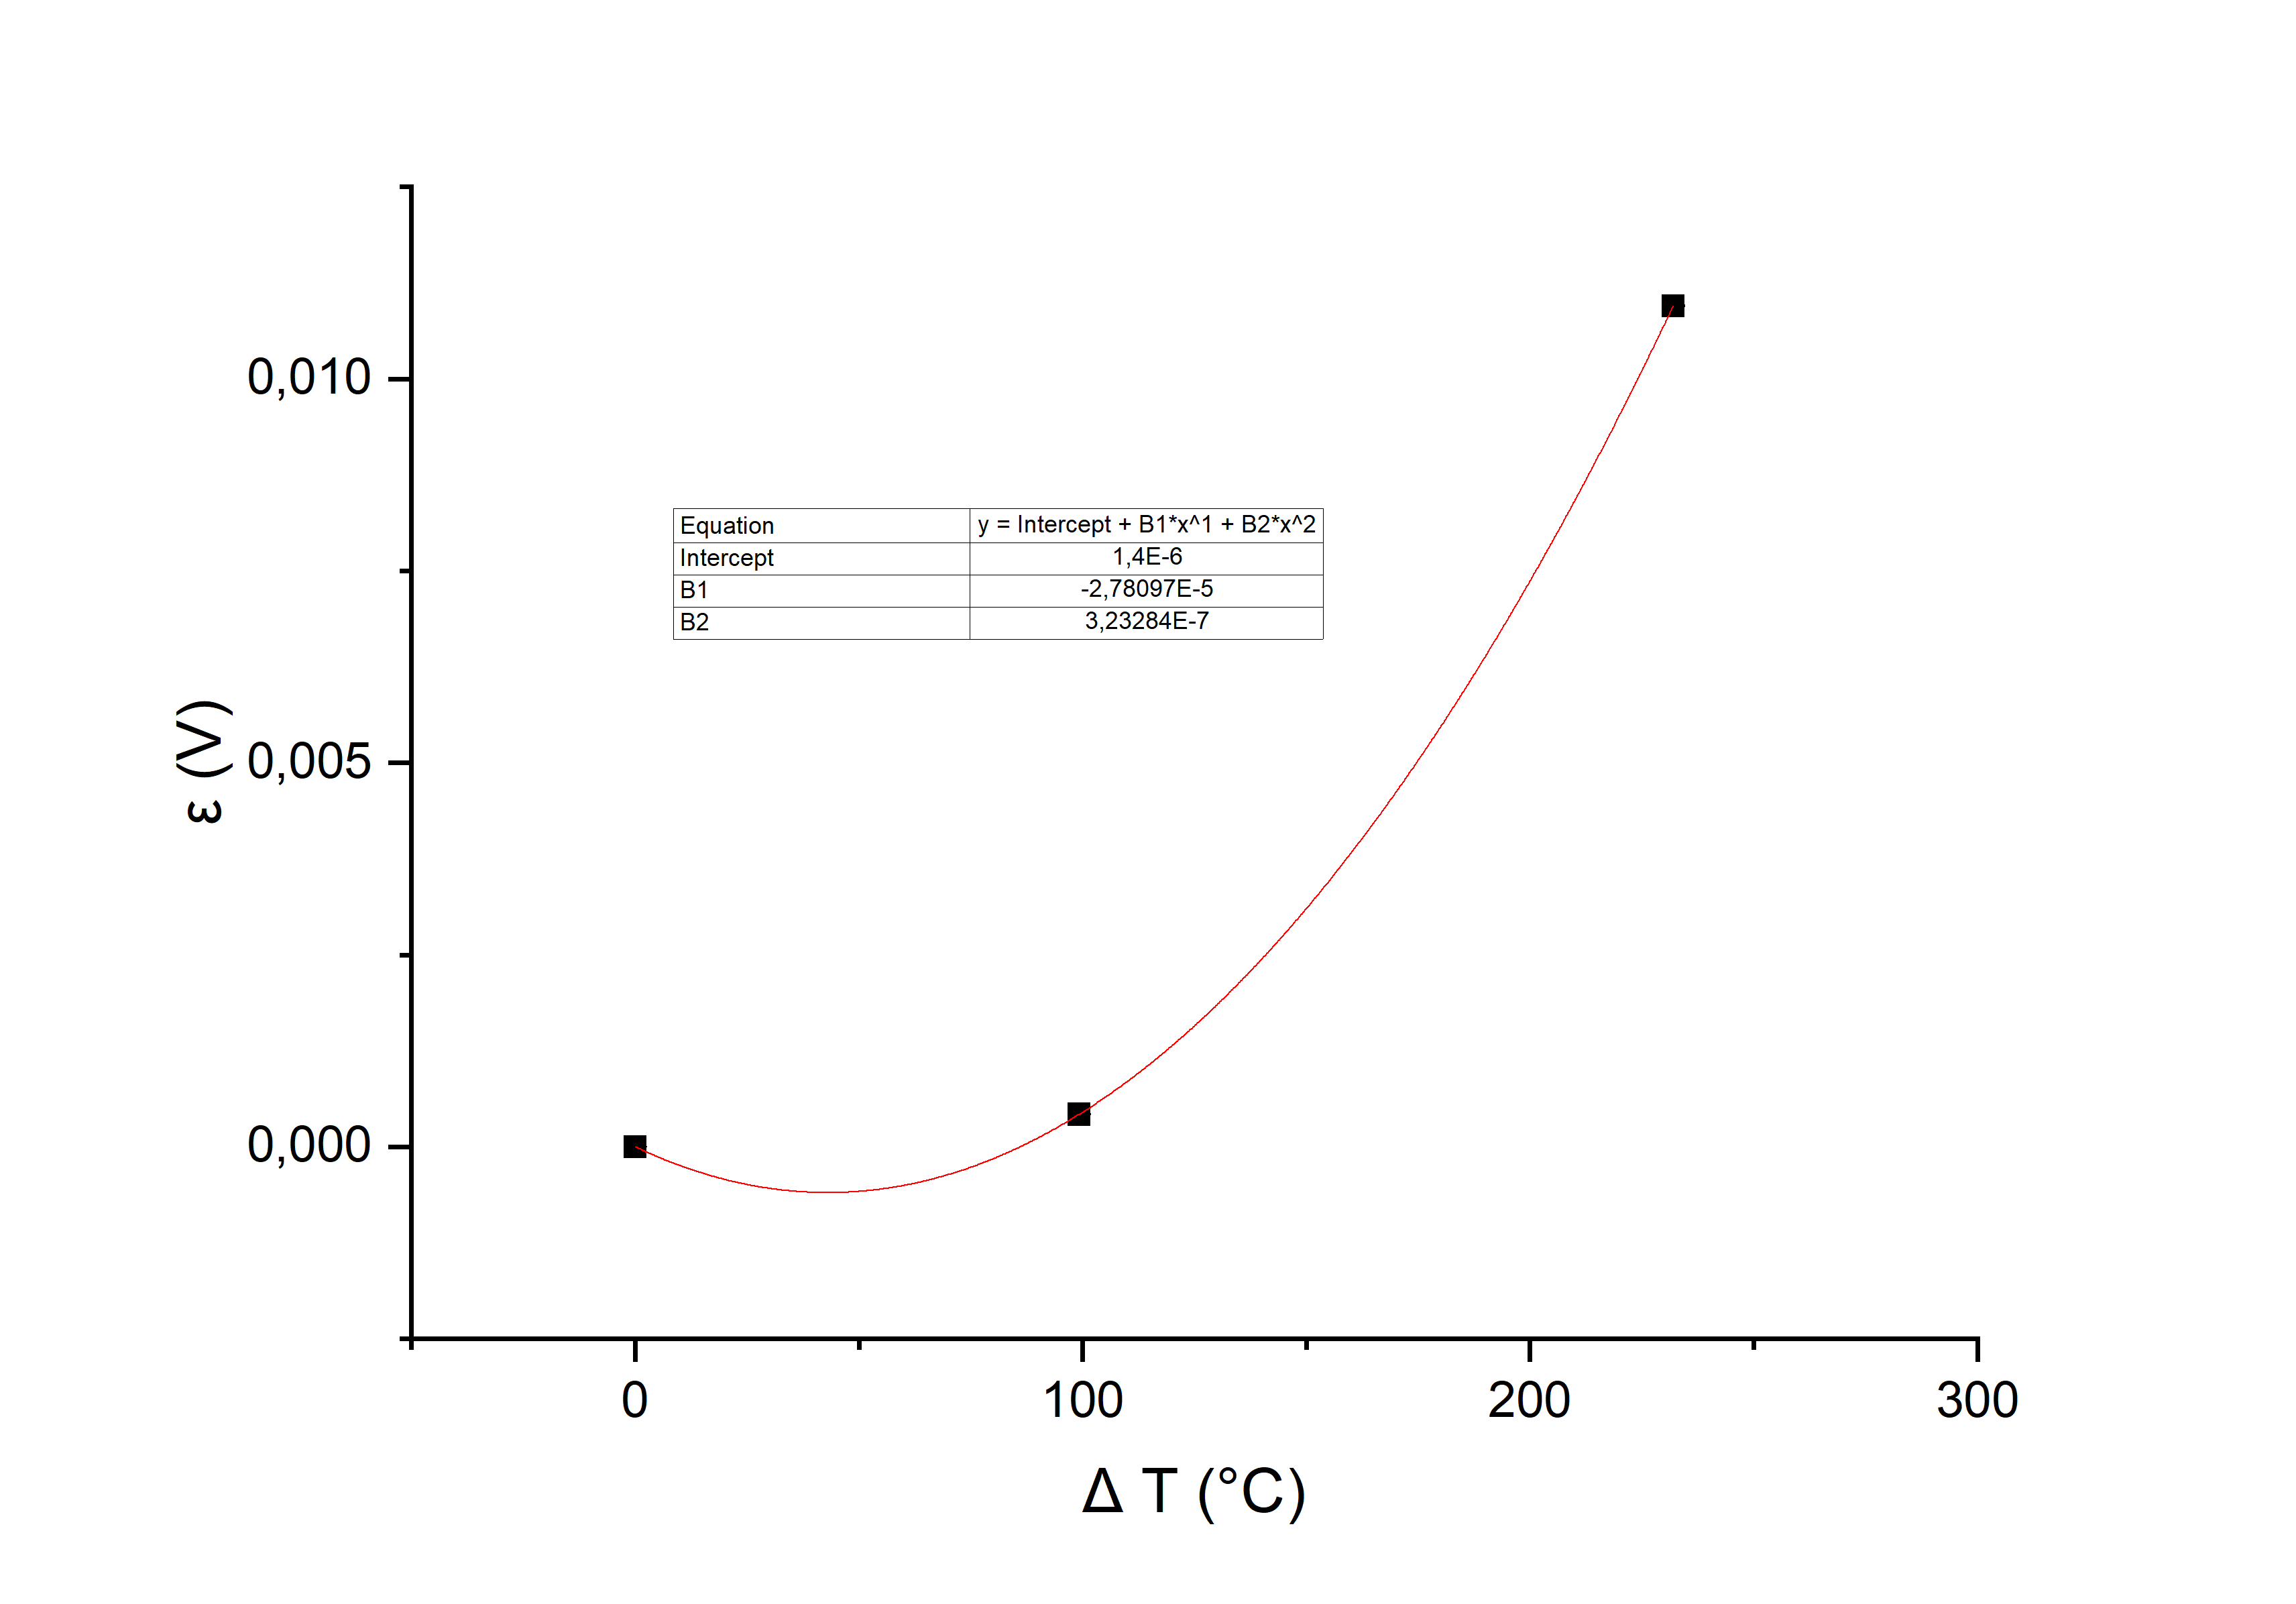
\includegraphics[width=0.8\linewidth]{8 - Kalibrace odporového teploměru a termočlánku//Prototkol - kalibrace teploměru//img/Závislost epsilon na delta T, parabola.png}
    \caption{Kalibrační křivka termočlánku}
    \label{fig:krivka-termoclanek}
\end{figure}

Po dosazení do rovnice (1) tedy máme

\begin{align*}
    a = 1,4(2) \cdot 10^{-6} \; V\\
    b = -2,8(1) \cdot 10^{-5} \; \frac{V}{^\circ C}\\
    c = 3,2(2) \cdot 10^{-7} \; \frac{V}{^\circ C^2} \\
\end{align*}

kde chyba koeficientů b, c je 5 \%.

Po dosazení do rovnice (2) dostáváme

\begin{align*}
    R_0 = 101,0(5) \; \Omega \\
    A = 0,38(2) \; \frac{1}{^\circ C} \\
    B = -2,9(1) \cdot 10^{-5} \; \frac{1}{^\circ C^2} \\
\end{align*}

kde chyba koeficientů A, B je opět 5 \%.

\newpage
% ----------------------------------------------------------------------
%  Diskuse výsledků
% ----------------------------------------------------------------------			
\section{Diskuse výsledků}

% ----------------------------------------------------------------------
%  Závěr
% ----------------------------------------------------------------------
\section{Závěr}
